\documentclass{article}
\usepackage[utf8]{inputenc}
\usepackage[T1]{fontenc}
\usepackage[francais]{babel}
\usepackage{lmodern}
\usepackage{graphicx}

\marginparwidth 0 pt
\oddsidemargin  0 pt
\evensidemargin  0 pt
\marginparsep 0 pt

\topmargin   0 pt

\textwidth   6.5 in
\textheight  8.5 in

\title{Feuille de route}
\author{Bollini Kevin, Mélia Geoffrey, Pagès Julien, Saleil Baptiste}
\date{21 Janvier 2012}

\begin{document}

\maketitle
	Nom du groupe : \textbf{PouerMouer} \\
	\ \\
	Composition du groupe et contact :
	\begin{itemize}
	\item Kevin Bollini : kevin.bollini@etud.univ-montp2.fr \\
	\item Geoffrey Mélia : geoffrey.melia@etud.univ-montp2.fr \\
	\item Julien Pagès : julien.pages01@etud.univ-montp2.fr \\
	\item Baptiste Saleil : baptiste.saleil@etud.univ-montp2.fr \\
	\end{itemize} 	

\section{Documents}
	Voici la liste des références et des différents documents à lire dans le cadre du TER. \\

	\subsection{Recherche}
	\begin{itemize}
		\item \it{Real-time viewpoint-invariant hand localization with cluttered backgrounds} \\
		Enver Sanginetoa, Marco Cupellib. \\
		http://www.sciencedirect.com.www.ezp.biu-montpellier.fr/science/article/pii/S026288561100120X
		\item \it{Vision par ordinateur pour l’interaction homme-machine fortement couplée}\\
		Thèse de françois Bérard sur un sujet proche avec beaucoup d'informations \\
		http://hal.inria.fr/docs/00/04/61/56/PDF/tel-00004804.pdf
		\item \it{Defining Search Areas to Localize Limbs in Body Motion Analysis} \\
		Thomas Foures, Philippe Joly. \\
		http://www.irit.fr/\textasciitilde Philippe.Joly/Homepage\_files/Articles/AMR03.pdf \\
	\end{itemize}

	\subsection{Programmation}
	Ces documents nous serviront à contruire notre application et à mieux cerner la problématique. \\	
	\begin{itemize}
		\item \it{Vision par ordinateur : Outils fondamentaux} \\
		Radu HORAUD (CNRS) et Olivier MONGA (INRIA) \\
		http://hal.archives-ouvertes.fr/docs/00/59/00/49/PDF/VO-HoraudMonga.pdf
		
		\item Learning Open CV \\
		 Gary Bradski et Adrian Kaehler
	\end{itemize}

	\section{Planning}
	\begin{center}
		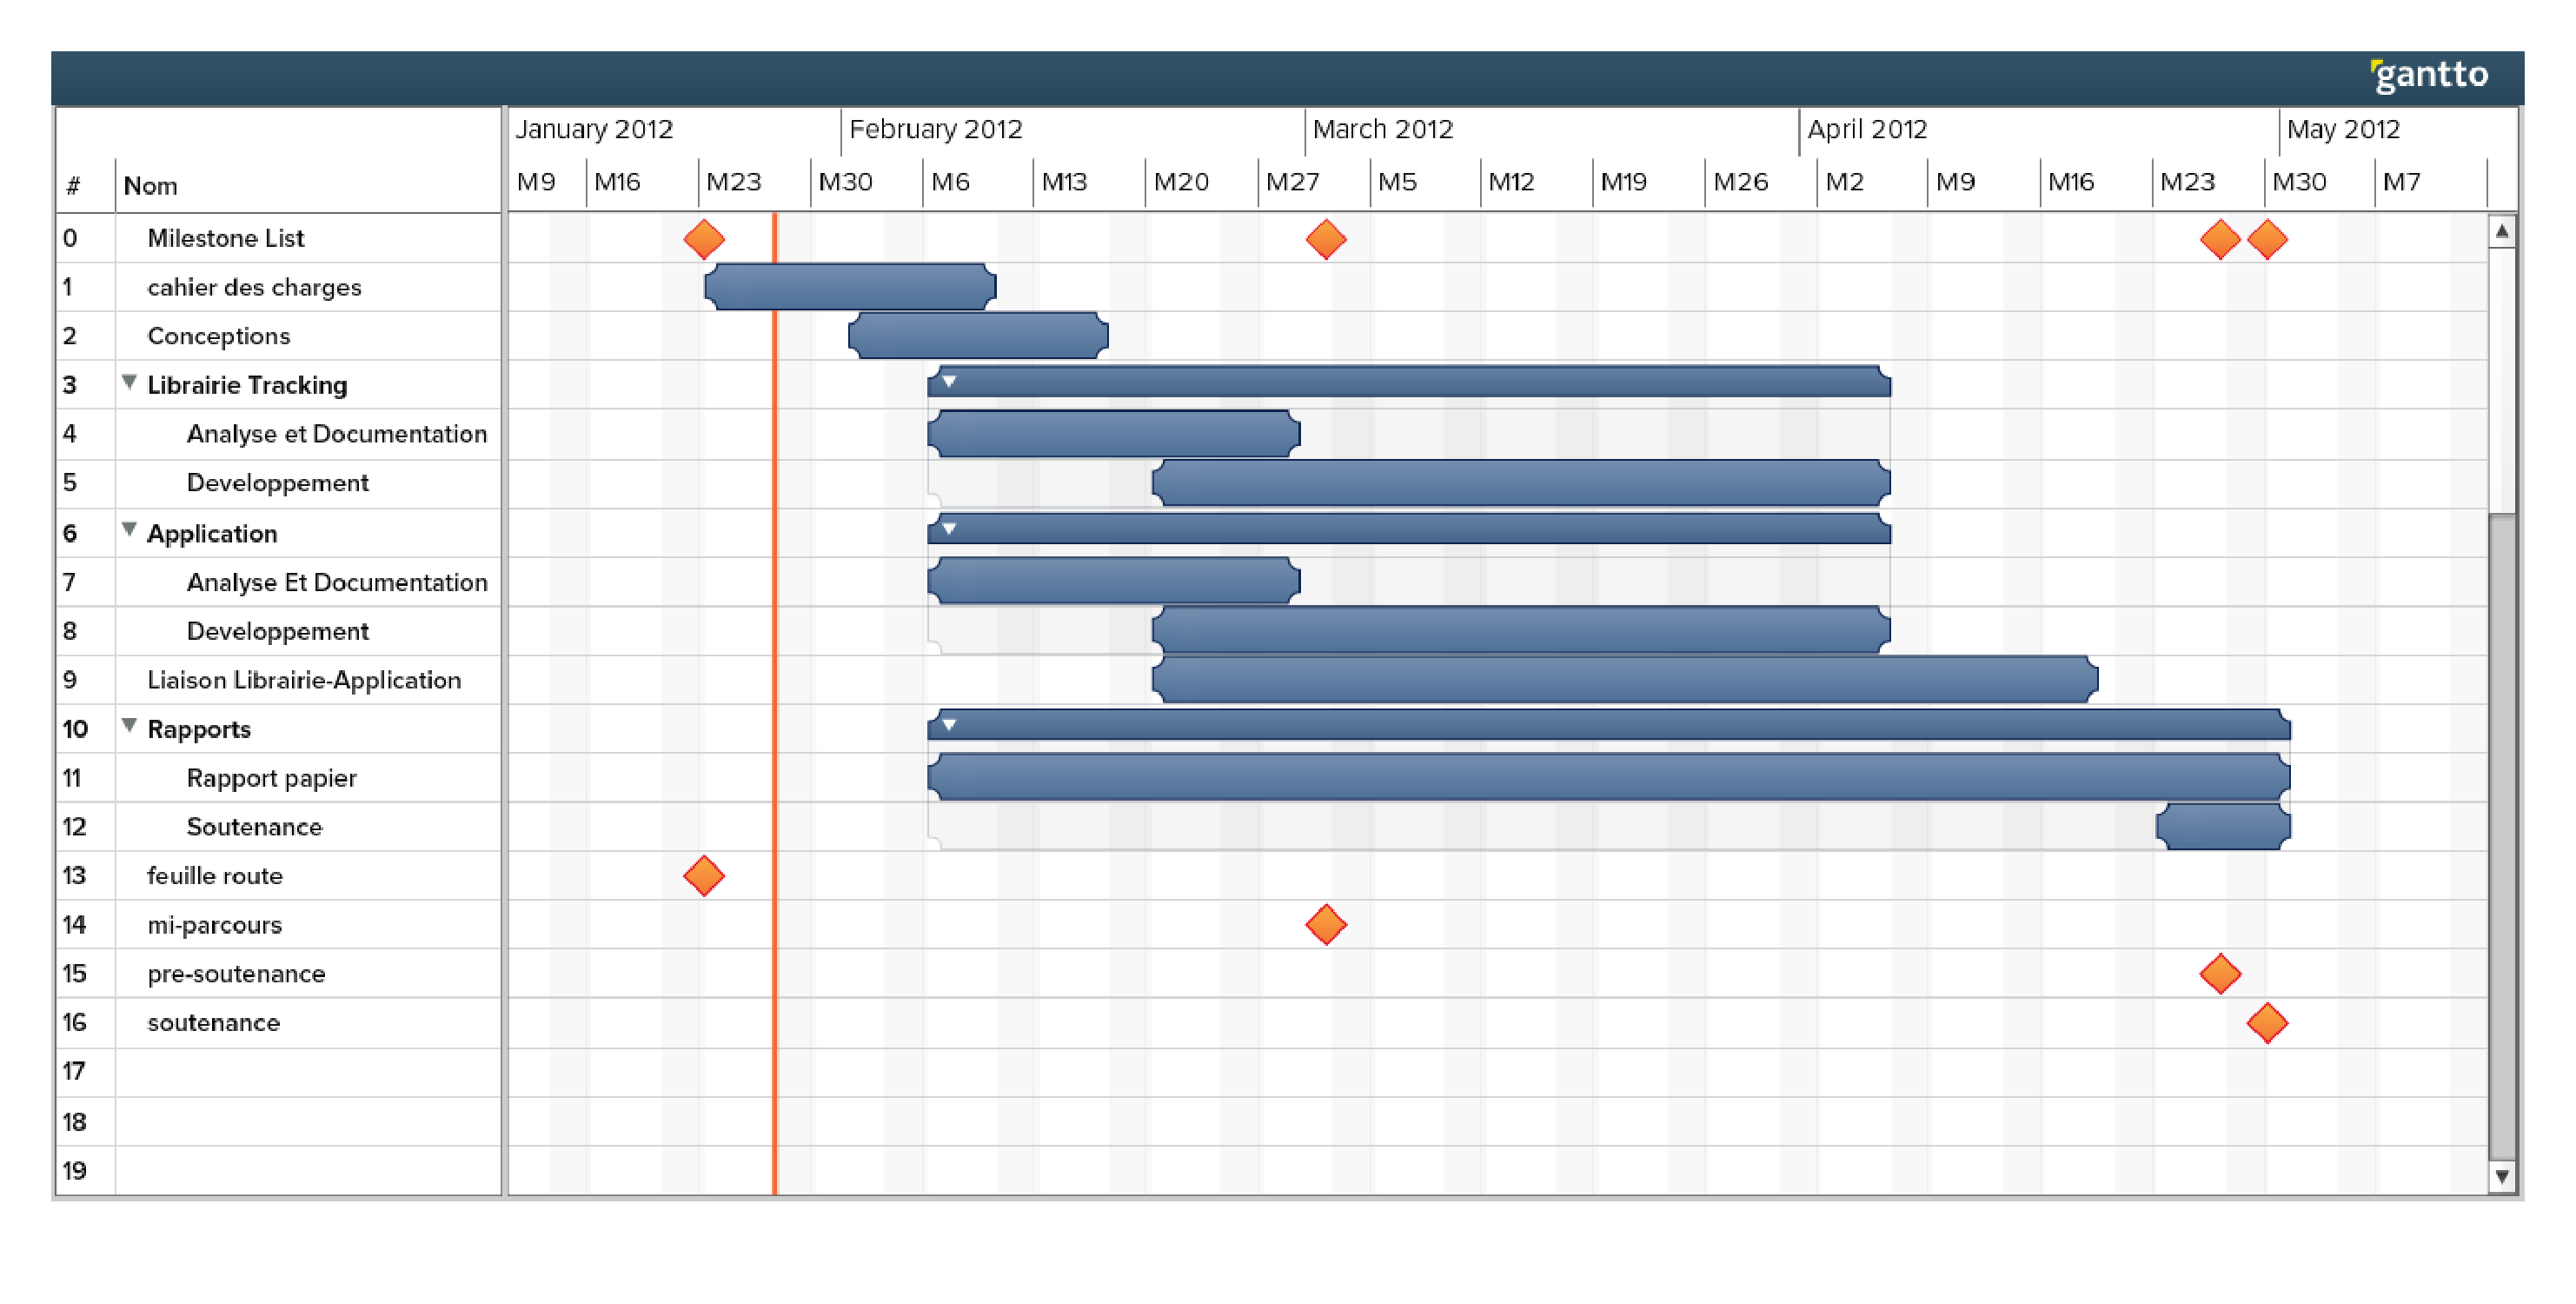
\includegraphics[scale=0.37]{retroplanning.pdf}
		\it rétro-planning
	\end{center}
	
	L'application étant découpée en deux parties majeures, l'attribution des tâches sera faite en fonction des spécialités.
	La partie développement du logiciel sera gérée par Julien Pagès et Baptiste Saleil (master AIGLE). \\
	La partie traitement de l'image avec le développement de la librairie sera gérée par kevin Bollini et Geoffrey Mélia 
	(master IMAGINA).	
\end{document}

